\documentclass[11pt]{scrartcl}

\title{Architektur}
\author{Silvan Adrian \\ Fabian Binna}
\date{\today{}}

\usepackage[ngerman]{babel}
\usepackage[automark]{scrpage2}
\usepackage[colorlinks = true,
linkcolor = black]{hyperref}
\usepackage{color}
\usepackage[normalem]{ulem}
\usepackage{scrpage2}
\usepackage{graphicx}
\usepackage{tabularx}
\graphicspath{ {../22_Grafiken/01_Logo/}{images/}{../../22_Grafiken/01_Logo/} }
\pagestyle{scrheadings}

\clearscrheadfoot
\ihead{
\includegraphics[scale=0.3]{SDDC}}
\ohead{Projekt: SDDC}
\ifoot{Architektur}
\cfoot{Version: 1.05}
\ofoot{Datum: \today{}}
\setheadsepline{0.5pt}
\setfootsepline{0.5pt}

\usepackage{ucs}
\usepackage[utf8]{inputenc}
\usepackage[T1]{fontenc}


\begin{document}
\def\arraystretch{1.5}
\begin{titlepage}
\begin{center}
\vspace{10em}

\includegraphics[scale=2]{SDDC}
\vspace{10em}
\end{center}
\begin{center}
\huge {Architektur}
\end{center}
\begin{center}
\vspace{10em}
\LARGE {Silvan Adrian} \\
\LARGE {Fabian Binna}
\end{center}

\end{titlepage}

\newpage
\section{Änderungshistorie}
\begin{tabularx}{\linewidth}{l l X l}
\textbf{Datum} & \textbf{Version} & \textbf{Änderung}  & \textbf{Autor} \\
\hline
\textbf{17.09.15} & 1.00 & Erstellung des Dokuments & Gruppe \\
\textbf{18.10.15} & 1.01 & Dokumentaufbau + Logische Sicht & Fabian Binna\\
\textbf{20.10.15} & 1.02 & Klassenstrukturen & Fabian Binna\\
\textbf{26.10.15} & 1.03 & Klassenstrukturen verbessert + Klassenstruktur genericapi & Fabian Binna\\
\textbf{14.11.15} & 1.04 & Datenmodell und Verbesserungen & Silvan Adrian\\
\textbf{22.11.15} & 1.05 & Logisch Architektur erneuert & Fabian Binna\\

\end{tabularx}

\newpage
\tableofcontents
\newpage

\subsection{Zweck}
Dieses Dokument beschreibt die Software Architektur für das Projekt SDDC.
\subsection{Gültigkeitsbereich}
Dieses Dokument ist während des ganzen Projekts gültig und wird laufend aktualisiert.

\newpage

\section{Systemübersicht}

\section{Logische Architektur}
\begin{itemize}
	\item services: Web-Schnittstelle (RESTful)
	\item genericapi: Abstraktion für Compute, Storage und Network
	\item common: DTOs (Service, OrderedService, ServiceModule)
	\item util: Tools zur Bearbeitung von Configfiles
	\item presistence: OR-Mapping
\end{itemize}

\begin{center}
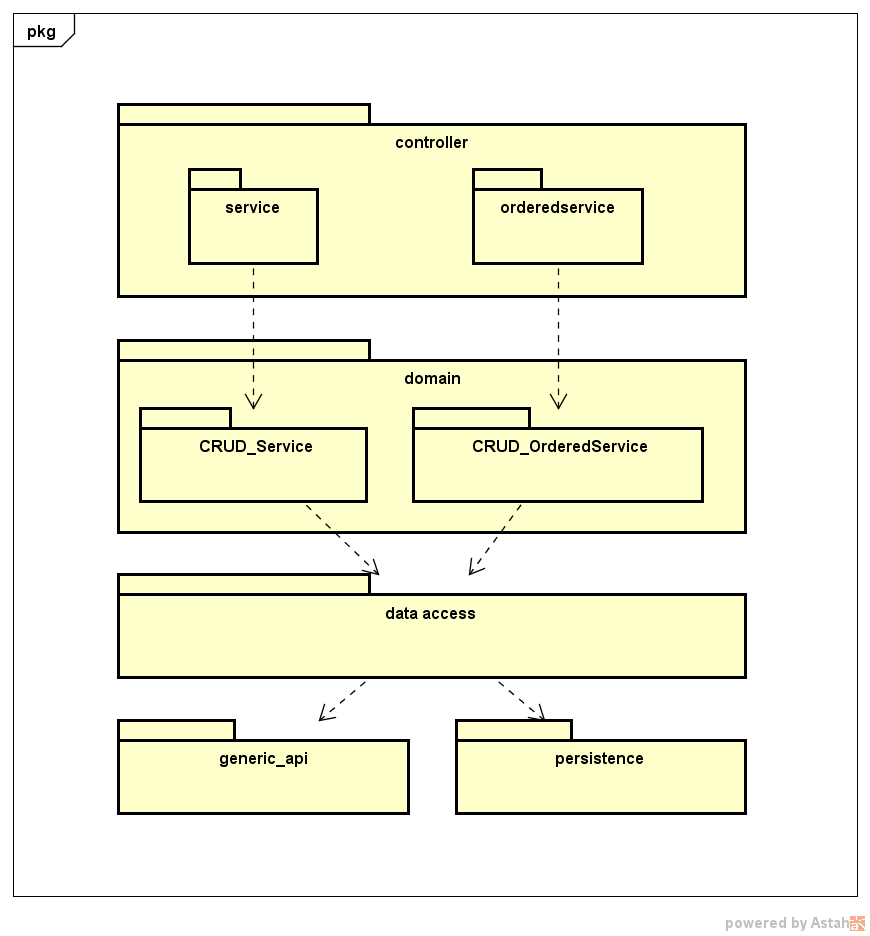
\includegraphics[scale=0.5]{LogischeSicht}
\end{center}

\newpage

\section{Klassenstruktur}



\subsection{persistence}

Wird durch OR Mapper (Hibernate) vorgenommen, dieser mappt die Java Objekte auf 
die Datenbank.

\section{Deployment}

\includegraphics[width=\textwidth]{deployment}

\section{Persistierung}

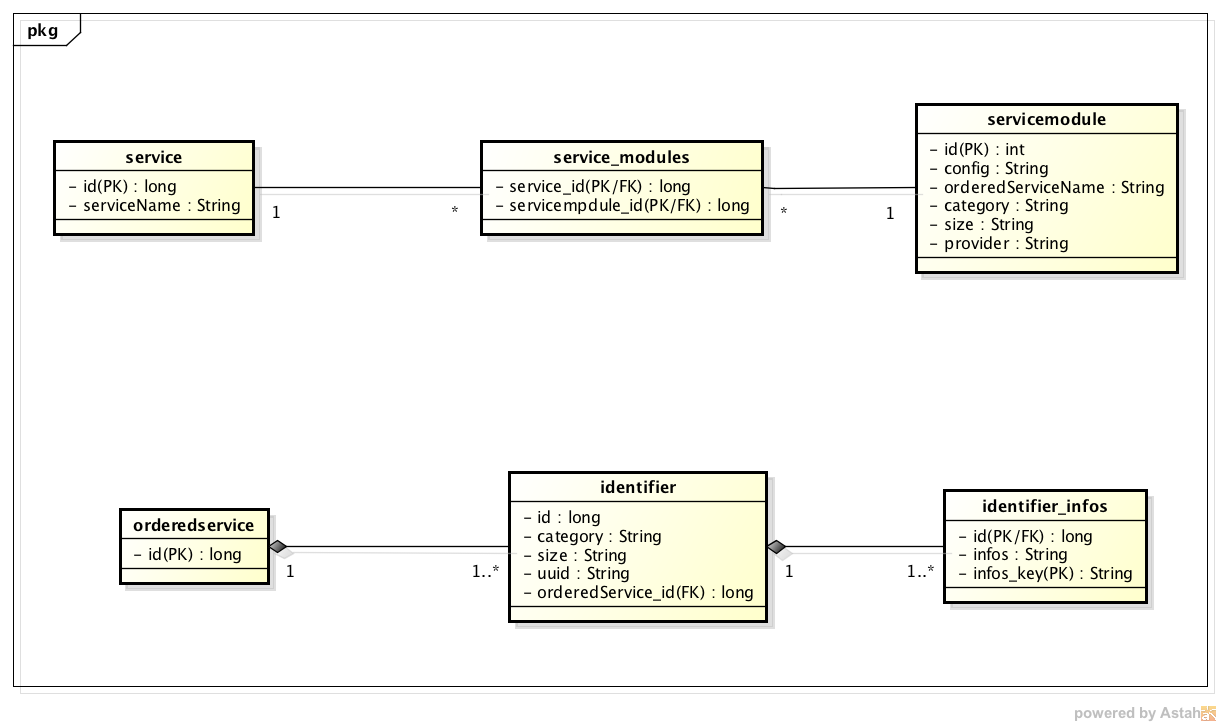
\includegraphics[width=\textwidth]{Datenmodell}








\end{document}